\gaokaoheader{2020}{浙江7月选考卷}

\gaokaoxz

\begin{enumerate}
%\renewcommand{\labelenumi}{\arabic{enumi}.}
% A(\Alph) a(\alph) I(\Roman) i(\roman) 1(\arabic)
%设定全局标号series=example	%引用全局变量resume=example
%[topsep=-0.3em,parsep=-0.3em,itemsep=-0.3em,partopsep=-0.3em]
%可使用leftmargin调整列表环境左边的空白长度 [leftmargin=0em]
\item
国际单位制中电荷量的单位符号是 $ C $,如果用国际单位制基本单位的符号来表示,正确的是 \xzanswer{B} 

\fourchoices
{$ F \cdot V $}
{$ A \cdot s $}
{$ J/V $}
{$ N \cdot m/V $}

%题目类型:
%题目区域:
%题目难度:
%思想方法:
%题目特征:

\item
如图所示,底部均有 $ 4 $ 个轮子的行李箱 $ a $ 竖立、$ b $ 平卧放置在公交车上,箱子四周有一定空间。当公交车 \xzanswer{B} 
% TODO: \usepackage{graphicx} required
\begin{figure}[h!]
\centering
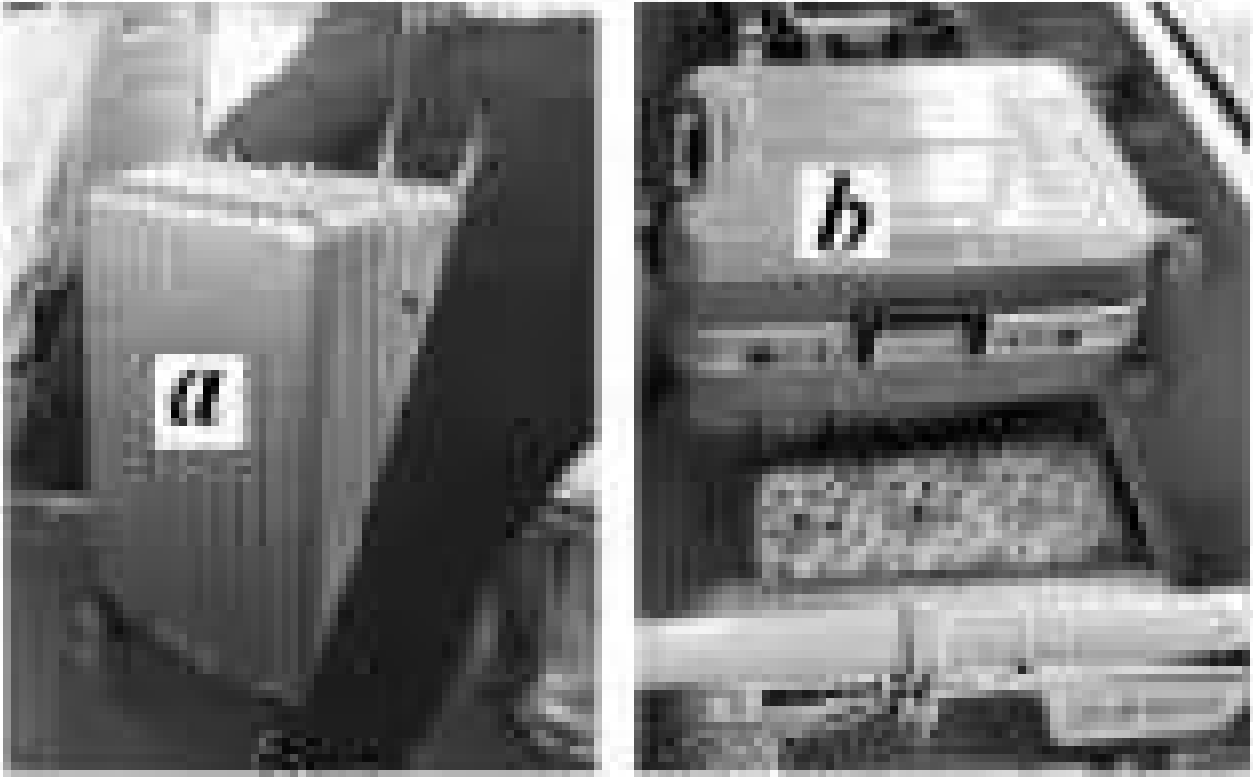
\includegraphics[width=0.23\linewidth]{picture/screenshot041}
\end{figure}

\fourchoices
{缓慢起动时,两只行李箱一定相对车子向后运动}
{急刹车时,行李箱 $ a $ 一定相对车子向前运动}
{缓慢转弯时,两只行李箱一定相对车子向外侧运动}
{急转弯时,行李箱 $ b $ 一定相对车子向内侧运动}

%题目类型:
%题目区域:
%题目难度:
%思想方法:
%题目特征:

\item
矢量发动机是喷口可向不同方向偏转以产生不同方向推力的一种发动机。当歼 $ 20 $ 隐形战斗机以速度 $ v $ 斜
向上飞行时,其矢量发动机的喷口如图所示。已知飞机受到重力 $ G $、发动机推力 $ F_{1} $、与速度方向垂直的升
力 $ F_{2} $ 和与速度方向相反的空气阻力 $ F_{f} $。下列受力分析示意图可能正确的是 \xzanswer{A} 
% TODO: \usepackage{graphicx} required
\begin{figure}[h!]
\centering
%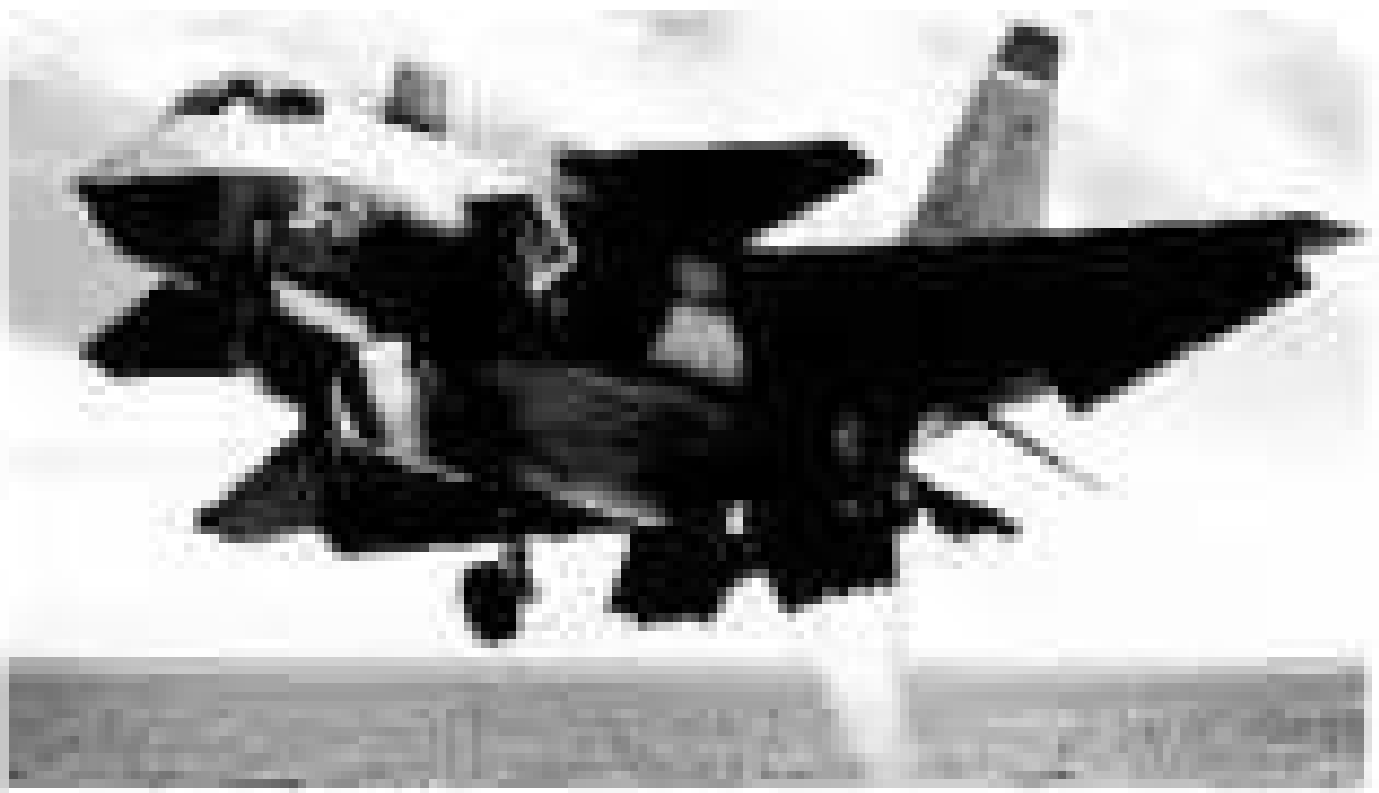
\includegraphics[width=0.2\linewidth]{picture/screenshot042}
 \includesvg[width=0.23\linewidth]{picture/svg/GZ-3-tiyou-0702} 
\end{figure}

\pfourchoices
{\includesvg[height=3cm]{picture/svg/GZ-3-tiyou-0698}}
{\includesvg[height=3cm]{picture/svg/GZ-3-tiyou-0699}}
{\includesvg[height=3cm]{picture/svg/GZ-3-tiyou-0700}}
{\includesvg[height=3cm]{picture/svg/GZ-3-tiyou-0701}}



%题目类型:
%题目区域:
%题目难度:
%思想方法:
%题目特征:


\item
在抗击新冠病毒的过程中,广泛使用了红外体温计测量体温,如图所示。下列说法正确的是 \xzanswer{D} 
% TODO: \usepackage{graphicx} required
\begin{figure}[h!]
\centering
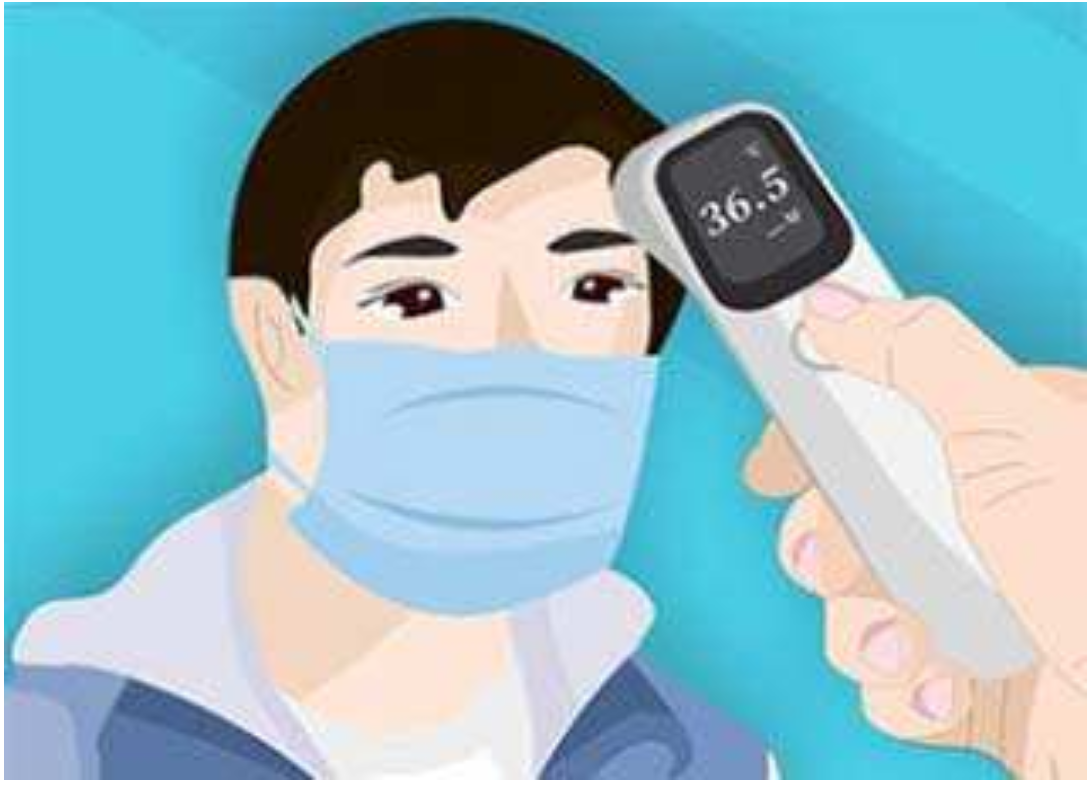
\includegraphics[width=0.2\linewidth]{picture/screenshot043}
%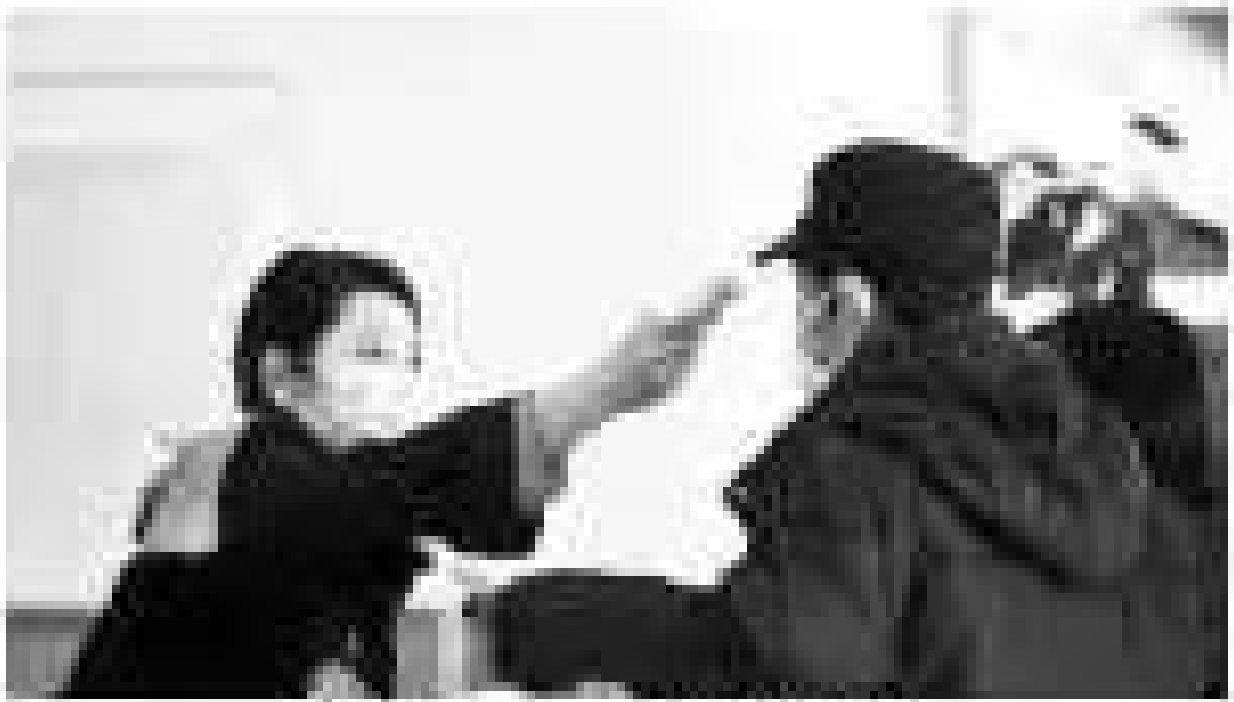
\includegraphics[width=0.2\linewidth]{picture/screenshot044}
\end{figure}


\fourchoices
{当体温超过 $ 37.3 \ \celsius $时人体才辐射红外线}
{当体温超过周围空气温度时人体才辐射红外线}
{红外体温计是依据体温计发射红外线来测体温的}
{红外体温计是依据人体温度越高,辐射的红外线强度越大来测体温的}


%题目类型:
%题目区域:
%题目难度:
%思想方法:
%题目特征:

\item
下列说法正确的是 \xzanswer{D} 


\fourchoices
{质子的德布罗意波长与其动能成正比}
{天然放射的三种射线,穿透能力最强的是 $ \alpha $ 射线}
{光电效应实验中的截止频率与入射光的频率有关}
{电子束穿过铝箔后的衍射图样说明电子具有波动性}

%题目类型:
%题目区域:
%题目难度:
%思想方法:
%题目特征:

\item
如图所示,一质量为 $ m $、电荷量为 $ q $ ( $ q>0 $ )的粒子以速度 $ v_{0} $ 从 $ MN $ 连线上的 $ P $ 点水平向右射入大小
为 $ E $、方向竖直向下的匀强电场中。已知 $ MN $ 与水平方向成 $ 45 ^{ \circ } $角,粒子的重力可以忽略,则粒子到达 $ MN $
连线上的某点时 \xzanswer{C} 
\begin{figure}[h!]
\centering
\includesvg[width=0.26\linewidth]{picture/svg/GZ-3-tiyou-0706}
\end{figure}


\fourchoices
{所用时间为$\frac{m v_{0}}{q E}$}
{速度大小为 $ 3 v_{0} $}
{与 $ P $ 点的距离为$\frac{2 \sqrt{2} m v_{0}^{2}}{q E}$}
{速度方向与竖直方向的夹角为 $ 30 ^{ \circ } $}

%题目类型:
%题目区域:
%题目难度:
%思想方法:
%题目特征:

\item
火星探测任务“天问一号”的标识如图所示。若火星和地球绕太阳的运动均可视为匀速圆周运动,火星
公转轨道半径与地球公转轨道半径之比为 $ 3:2 $,则火星与地球绕太阳运动的 \xzanswer{C} 
% TODO: \usepackage{graphicx} required
\begin{figure}[h!]
\centering

\includegraphics[width=0.17\linewidth]{picture/screenshot045}
\end{figure}


\fourchoices
{轨道周长之比为 $ 2:3 $}
{线速度大小之比为 $ \sqrt{3} : \sqrt{2} $}
{角速度大小之比为 $2 \sqrt{2}: 3 \sqrt{3}$}
{向心加速度大小之比为 $ 9:4 $}

%题目类型:
%题目区域:
%题目难度:
%思想方法:
%题目特征:



\item
空间 $ P $、$ Q $ 两点处固定电荷量绝对值相等的点电荷,其中 $ Q $ 点处为正电荷,$ P $、$ Q $ 两点附近电场的等势线
分布如图所示,$ a $、$ b $、$ c $、$ d $、$ e $ 为电场中的 $ 5 $ 个点,设无穷远处电势为 $ 0 $,则 \xzanswer{D} 
\begin{figure}[h!]
\centering
\includesvg[width=0.23\linewidth]{picture/svg/GZ-3-tiyou-0708}
\end{figure}



\fourchoices
{$ e $ 点的电势大于 $ 0 $}
{$ a $ 点和 $ b $ 点的电场强度相同}
{$ b $ 点的电势低于 $ d $ 点的电势}
{负电荷从 $ a $ 点移动到 $ c $ 点时电势能增加}

%题目类型:
%题目区域:
%题目难度:
%思想方法:
%题目特征:



\item
特高压直流输电是国家重点能源工程。如图所示,两根等高、相互平行的水平长直导线分别通有方向相
同的电流 $ I_{1} $ 和 $ I_{2} $, $ I_{1} > I_{2} $。$ a $、$ b $、$ c $ 三点连线与两根导线等高并垂直,$ b $ 点位于两根导线间的中点,$ a $、$ c $
两点与 $ b $ 点距离相等,$ d $ 点位于 $ b $ 点正下方。不考虑地磁场的影响,则 \xzanswer{C} 
% TODO: \usepackage{graphicx} required
\begin{figure}[h!]
\centering
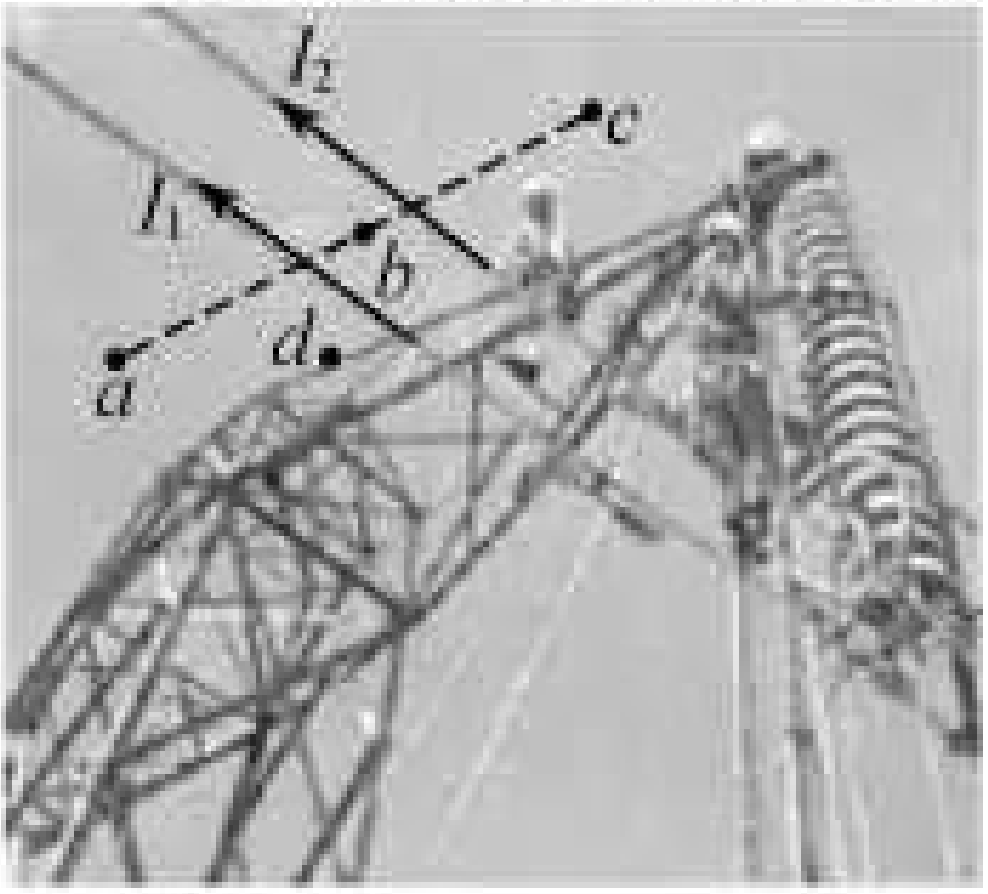
\includegraphics[width=0.2\linewidth]{picture/screenshot046}
%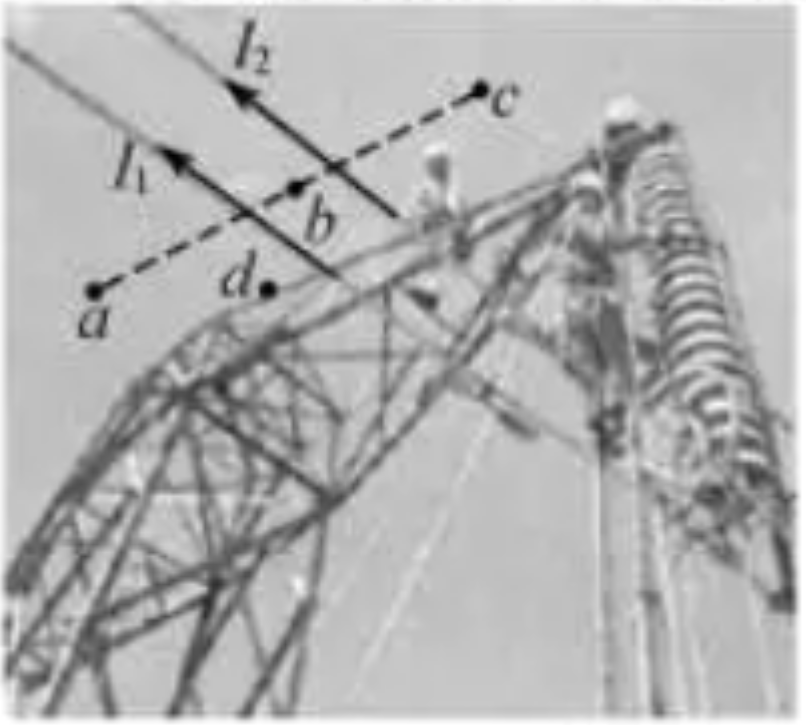
\includegraphics[width=0.2\linewidth]{picture/screenshot048}
\end{figure}



\fourchoices
{$ b $ 点处的磁感应强度大小为 $ 0 $}
{$ d $ 点处的磁感应强度大小为 $ 0 $}
{$ a $ 点处的磁感应强度方向竖直向下}
{$ c $ 点处的磁感应强度方向竖直向下}

%题目类型:
%题目区域:
%题目难度:
%思想方法:
%题目特征:


\item
如图是“中国天眼” $ 500 \ m $ 口径球面射电望远镜维护时的照片。为不损伤望远镜球面,质量为 $ m $ 的工作
人员被悬在空中的氦气球拉着,当他在离底部有一定高度的望远镜球面上缓慢移动时,氦气球对其有大小为
$ \frac{ 5 }{ 6 } mg $、方向竖直向上的拉力作用,使其有“人类在月球上行走”的感觉,若将人视为质点,此时工作人员 \xzanswer{D} 
% TODO: \usepackage{graphicx} required
\begin{figure}[h!]
\centering
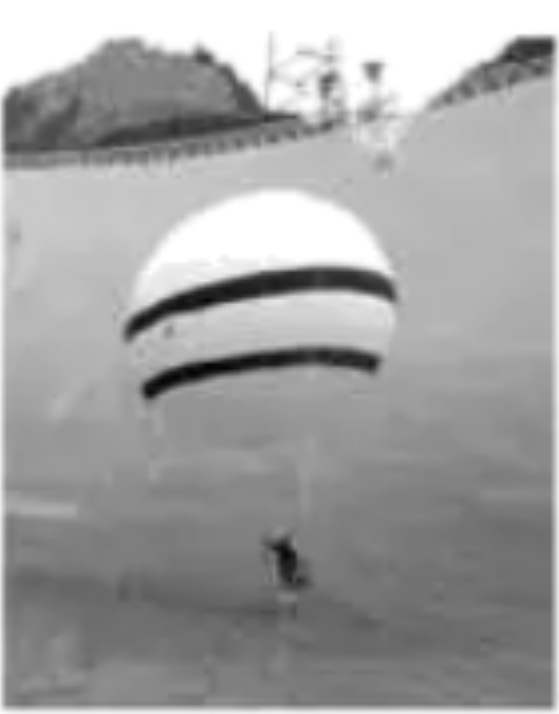
\includegraphics[width=0.15\linewidth]{picture/screenshot047}
\end{figure}


\fourchoices
{受到 的重力大小为 $ \frac{ 1 }{ 6 } mg $}
{受到的合力大小为 $ \frac{ 1 }{ 6 } mg $}
{对球面的压力大小为 $ \frac{ 1 }{ 6 } mg $}
{对球面的作用力大小为 $ \frac{ 1 }{ 6 } mg $}

%题目类型:
%题目区域:
%题目难度:
%思想方法:
%题目特征:

\item
如图所示,某小型水电站发电机的输出功率 $ P=100 \ kW $,发电机的电压 $ U_{1} =250 \ V $,经变压器升压后
向远处输电,输电线总电阻 $ R _{ \text{线} } =8 \ \Omega $,在用户端用降压变压器把电压降为 $ U_4=220 \ V $。已知输电线上损失
的功率 $ P _{ \text{线} } =5 \ kW $,假设两个变压器均是理想变压器,下列说法正确的是 \xzanswer{C} 
\begin{figure}[h!]
\centering
\includesvg[width=0.6\linewidth]{picture/svg/GZ-3-tiyou-0709}
\end{figure}


\fourchoices
{发电机输出的电流 $ I_{1} =40 \ A $}
{输电线上的电流 $ I_{ \text{线} }=625 \ A $}
{降压变压器的匝数比 $ n_{3}:n_4=190:11 $}
{用户得到的电流 $ I_4=455 \ A $}


%题目类型:
%题目区域:
%题目难度:
%思想方法:
%题目特征:

\item
如图所示,固定在水平面上的半径为 $ r $ 的金属圆环内存在方向竖直向上、磁感应强度大小为 $ B $ 的匀强磁
场。长为 $ l $ 的金属棒,一端与圆环接触良好,另一端固定在竖直导电转轴 $ OO ^{\prime} $ 上,随轴以角速度 $ \omega $ 匀速转
动。在圆环的 $ A $ 点和电刷间接有阻值为 $ R $ 的电阻和电容为 $ C $、板间距为 $ d $ 的平行板电容器,有一带电微粒
在电容器极板间处于静止状态。已知重力加速度为 $ g $,不计其它电阻和摩擦,下列说法正确的是 \xzanswer{B} 
\begin{figure}[h!]
\centering
\includesvg[width=0.33\linewidth]{picture/svg/GZ-3-tiyou-0710}
\end{figure}


\fourchoices
{棒产生的电动势为$\frac{1}{2} B l^{2} \omega$}
{微粒的电荷量与质量之比为$\frac{2 g d}{B r^{2} \omega}$}
{电阻消耗的电功率为$\frac{\pi B^{2} r^{4} \omega}{2 R}$}
{电容器所带 的电荷量为$C B r^{2} \omega$}

%题目类型:
%题目区域:
%题目难度:
%思想方法:
%题目特征:

\item
如图所示,圆心为 $ O $、半径为 $ R $ 的半圆形玻璃砖置于水平桌面上,光线从 $ P $ 点垂直界面入射后,恰好在
玻璃砖圆形表面发生全反射;当入射角 $ \theta=60 ^{ \circ } $ 时,光线从玻璃砖圆形表面出射后恰好与入射光平行。已知
真空中的光速为 $ c $,则 \xzanswer{C} 
\begin{figure}[h!]
\centering
\includesvg[width=0.3\linewidth]{picture/svg/GZ-3-tiyou-0711}
\end{figure}


\fourchoices
{玻璃砖的折射率为 $ 1.5 $}
{$ OP $ 之间的距离为$\frac{\sqrt{2}}{2} R$}
{光在玻璃砖内的传播速度为$\frac{\sqrt{3}}{3} c$}
{光从玻璃到空气的临界角为 $ 30 ^{ \circ } $}

%题目类型:
%题目区域:
%题目难度:
%思想方法:
%题目特征:

%二、选择题$ \lmd{2} $(本题共 $ 3 $ 小题,每小题 $ 2 $ 分,共 $ 6 $ 分。每小题列出的四个备选项中至少有一个是符合题目要求的。全部选对的得 $ 2 $ 分,选对但不全的得 $ 1 $ 分,有选错的得 $ 0 $ 分)


\item
太阳辐射的总功率约为 $ 4 \times 10^{26} \ W $,其辐射的能量来自于聚变反应。在聚变反应中,一个质量为
$ 1876.1 \ MeV/c^{2} $ ($ c $ 为真空中的光速)的氘核( \ce{^{2}_{1}H} )和一个质量为 $ 2809.5 \ MeV/c^{2} $ 的氚核( \ce{^{3}_{1}H} )结合
为一个质量为 $ 3728.4 \ MeV/c^{2} $ 的氦核( \ce{^{4}_{2}He} ),并放出一个 \ce{X} 粒子,同时释放大约 $ 17.6 \ MeV $ 的能量。下
列说法正确的是 \xzanswer{BC} 



\fourchoices
{\ce{X} 粒子是质子}
{\ce{X} 粒子的质量为 $ 939.6 \ MeV/c^{2} $}
{太阳每秒因为辐射损失的质量约为 $ 4.4 \times 10^9 \ kg $}
{太阳每秒因为辐射损失的质量约为 $ 17.6 \ MeV/c^{2} $}

%题目类型:
%题目区域:
%题目难度:
%思想方法:
%题目特征:

\item
如图所示,$ x $ 轴上 $ -2 \ m $、$ 12 \ m $ 处有两个振动周期均为 $ 4 \ s $、振幅均为 $ 1 \ cm $ 的相同的波源 $ S_{1} $、$ S_{2} $,$ t=0 $ 时
刻同时开始竖直向下振动,产生波长均为 $ 4 \ m $ 沿 $ x $ 轴传播的简谐横波。$ P $、$ M $、$ Q $ 分别是 $ x $ 轴上 $ 2 \ m $、 $ 5 \ m $ 和
$ 8.5 \ m $ 的三个点,下列说法正确的是 \xzanswer{CD} 
\begin{figure}[h!]
\centering
\includesvg[width=0.63\linewidth]{picture/svg/GZ-3-tiyou-0712}
\end{figure}


\fourchoices
{$ 6.0 \ s $ 时 $ P $、$ M $、$ Q $ 三点均已振动}
{$ 8.0 \ s $ 后 $ M $ 点的位移始终是 $ 2 \ cm $}
{$ 10.0 \ s $ 后 $ P $ 点的位移始终是 $ 0 $}
{$ 10.5 \ s $ 时 $ Q $ 点的振动方向竖直向下}

%题目类型:
%题目区域:
%题目难度:
%思想方法:
%题目特征:


\item
如图所示,系留无人机是利用地面直流电源通过电缆供电的无人机,旋翼由电动机带动。现有质量为$ 20 \ kg $、额定功率为 $ 5 \ kW $ 的系留无人机从地面起飞沿竖直方向上升,经过 $ 200 \ s $ 到达 $ 100 \ m $ 高处后悬停并进
行工作。已知直流电源供电电压为 $ 400 \ V $,若不计电缆的质量和电阻,忽略电缆对无人机的拉力,则 \xzanswer{BD} 
\begin{figure}[h!]
\centering
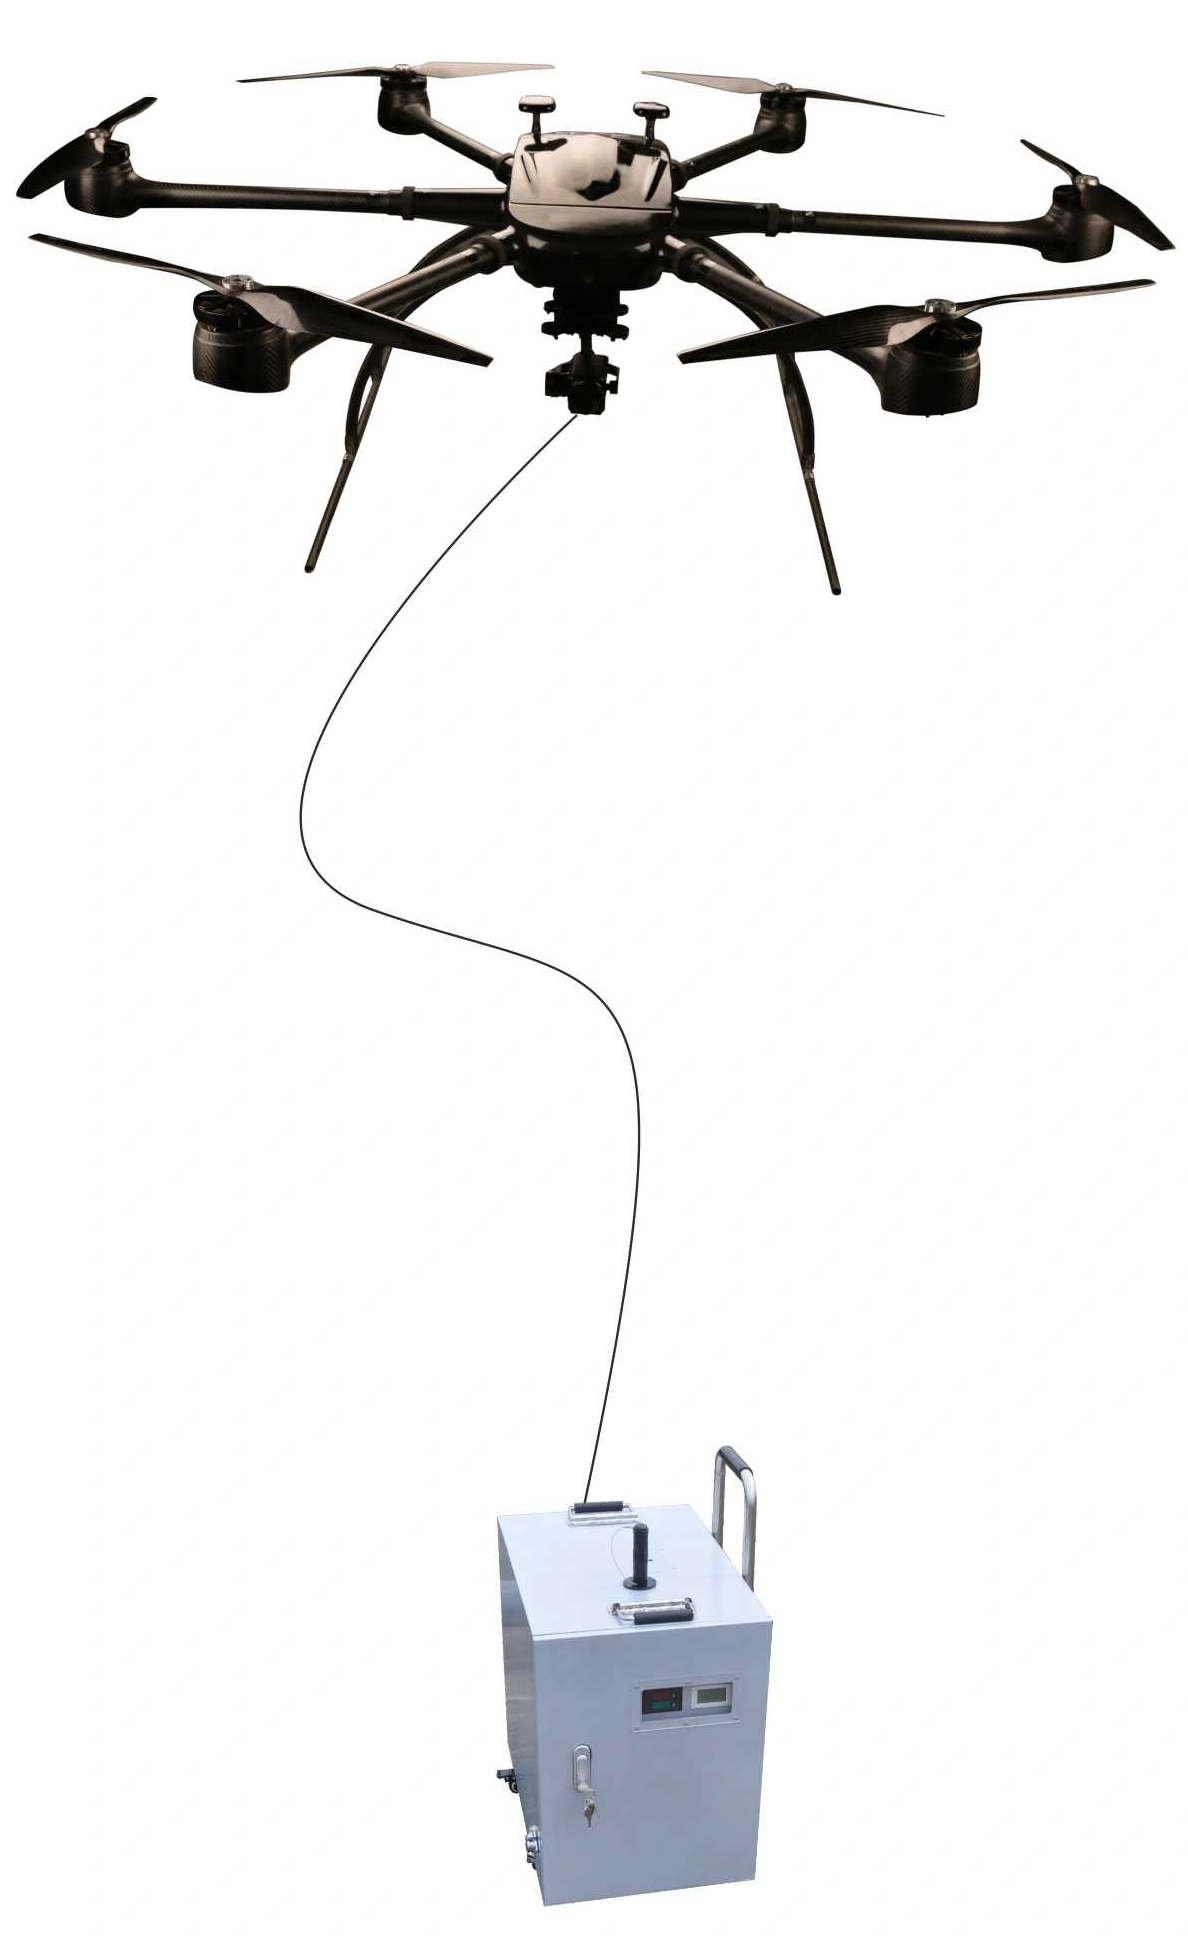
\includegraphics[width=0.15\linewidth]{picture/screenshot049}
\end{figure}

\fourchoices
{空气对无人机 的作用力始终大于或等于 $ 200 \ N $}
{直流电源对无人机供电的额定电流为 $ 12.5 \ A $}
{无人机上升过程中消耗的平均功率为 $ 100 \ W $}
{无人机上升及悬停时均有部分功率用于对空气做功}

%题目类型:
%题目区域:
%题目难度:
%思想方法:
%题目特征:


%三、非选择题(本题共 $ 6 $ 小题,共 $ 55 $ 分)



\item
做“探究加速度与力、质量的关系”实验时,图$ a $是教材中的实验方案;图$ b $是拓展方案,其实验操作
步骤如下:
\begin{figure}[h!]
\centering
\begin{subfigure}{0.44\linewidth}
\centering
\includesvg[width=0.9\linewidth]{picture/svg/GZ-3-tiyou-0716} 
\caption{}\label{}
\end{subfigure}
\begin{subfigure}{0.44\linewidth}
\centering
\includesvg[width=0.8\linewidth]{picture/svg/GZ-3-tiyou-0717} 
\caption{}\label{}
\end{subfigure}
\end{figure}
\begin{enumerate}
\renewcommand{\labelenumii}{\roman{enumii}.}
% A(\Alph) a(\alph) I(\Roman) i(\roman) 1(\arabic)
%设定全局标号series=example	%引用全局变量resume=example
%[topsep=-0.3em,parsep=-0.3em,itemsep=-0.3em,partopsep=-0.3em]
%可使用leftmargin调整列表环境左边的空白长度 [leftmargin=0em]
\item
挂上托盘和砝码,改变木板的倾角,使质量为 $ M $ 的小车拖着纸带沿木板匀速下滑;
\item 
取下托盘和砝码,测出其总质量为 $ m $,让小车沿木板下滑,测出加速度 $ a $;
\item 
改变砝码质量和木板倾角,多次测量,通过作图可得到 $ a-F $ 的关系。


\end{enumerate}

\begin{enumerate}
%\renewcommand{\labelenumi}{\arabic{enumi}.}
% A(\Alph) a(\alph) I(\Roman) i(\roman) 1(\arabic)
%设定全局标号series=example	%引用全局变量resume=example
%[topsep=-0.3em,parsep=-0.3em,itemsep=-0.3em,partopsep=-0.3em]
%可使用leftmargin调整列表环境左边的空白长度 [leftmargin=0em]
\item
实验获得如图所示的纸带,计数点 $ a $、$ b $、$ c $、$ d $、$ e $、$ f $ 间均有四个点未画出,则在打 $ d $ 点时小车的速度大
小 $ v_d=$ \underlinegap $ m/s $ (保留两位有效数字);
\begin{figure}[h!]
\centering
\includesvg[width=0.6\linewidth]{picture/svg/GZ-3-tiyou-0718}
\end{figure}

\item 
需要满足条件 $ M \gg m $ 的方案是 \underlinegap (选填“$ a $”、“$ b $”或“$ a $和$ b $”);在作 $ a-F $ 图象时,把 $ mg $作为 $ F $ 值的是 \underlinegap (选填“$ a $”、“$ b $”或“$ a $和$ b $”)。



\end{enumerate}


\tk{
\begin{enumerate}
%\renewcommand{\labelenumi}{\arabic{enumi}.}
% A(\Alph) a(\alph) I(\Roman) i(\roman) 1(\arabic)
%设定全局标号series=example	%引用全局变量resume=example
%[topsep=-0.3em,parsep=-0.3em,itemsep=-0.3em,partopsep=-0.3em]
%可使用leftmargin调整列表环境左边的空白长度 [leftmargin=0em]
\item
$0.18 \sim 0.19$
\item 
$ a $
\item 
$ a $和$ b $

\end{enumerate}
} 

%题目类型:
%题目区域:
%题目难度:
%思想方法:
%题目特征:


\item
某同学用单摆测量重力加速度。
\begin{enumerate}
%\renewcommand{\labelenumi}{\arabic{enumi}.}
% A(\Alph) a(\alph) I(\Roman) i(\roman) 1(\arabic)
%设定全局标号series=example	%引用全局变量resume=example
%[topsep=-0.3em,parsep=-0.3em,itemsep=-0.3em,partopsep=-0.3em]
%可使用leftmargin调整列表环境左边的空白长度 [leftmargin=0em]
\item
为了减少测量误差,下列做法正确的是 \underlinegap (多选);
\fourchoices
{摆的振幅越大越好}
{摆球质量大些、体积小些}
{摆线尽量细些、长些、伸缩性小些}
{计时的起、止位置选在摆球达到的最高点处}

\item 
改变摆长,多次测量,得到周期平方与摆长的关系图象如图所示,所得结果与当地重力加速度值相符,
但发现其延长线没有过原点,其原因可能是 \underlinegap 。
\begin{figure}[h!]
\centering
\includesvg[width=0.2\linewidth]{picture/svg/GZ-3-tiyou-0719}
\end{figure}

\fourchoices
{测周期时多数了一个周期}
{测周期时少数了一个周期}
{测摆长时直接将摆线的长度作为摆长}
{测摆长时将摆线的长度加上摆球的直径作为摆长}


\end{enumerate}

\tk{
\begin{enumerate}
%\renewcommand{\labelenumi}{\arabic{enumi}.}
% A(\Alph) a(\alph) I(\Roman) i(\roman) 1(\arabic)
%设定全局标号series=example	%引用全局变量resume=example
%[topsep=-0.3em,parsep=-0.3em,itemsep=-0.3em,partopsep=-0.3em]
%可使用leftmargin调整列表环境左边的空白长度 [leftmargin=0em]
\item
BC	
\item 
C	
\end{enumerate}
} 



\newpage
\item
某同学分别用图$ a $和图$ b $的电路测量同一节干电池的电动势和内阻。
\begin{figure}[h!]
\centering
\begin{subfigure}{0.4\linewidth}
\centering
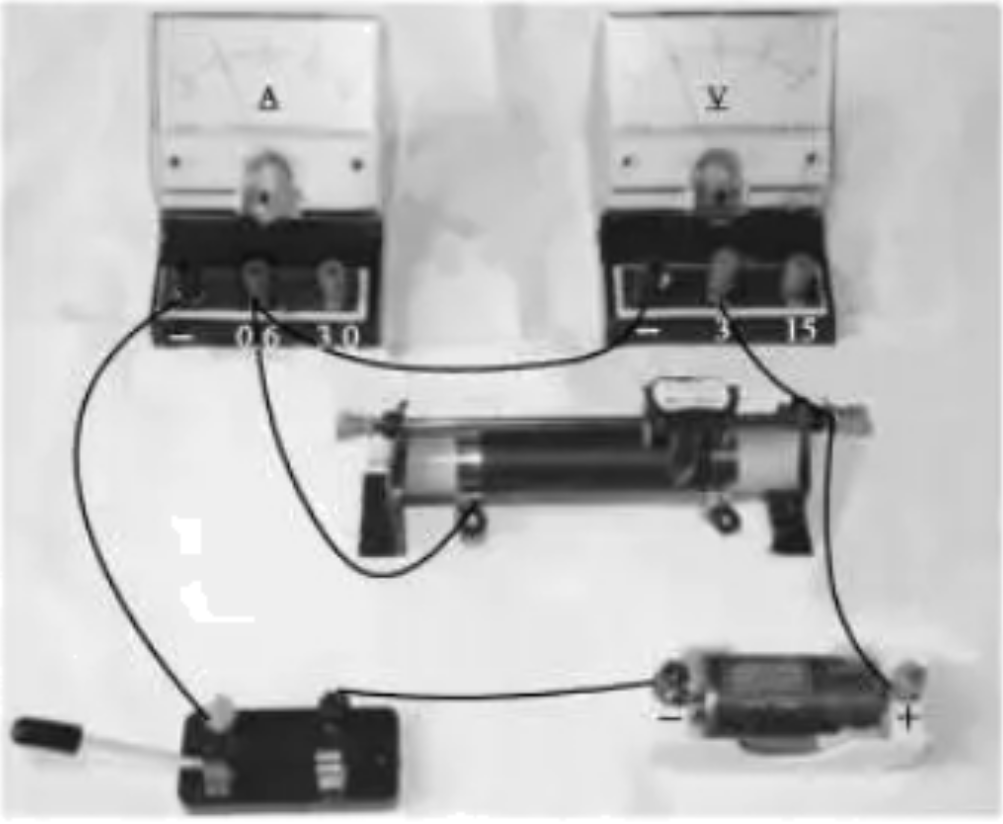
\includegraphics[width=0.9\linewidth]{picture/screenshot050}
\caption{}\label{}
\end{subfigure}
\hfil
\begin{subfigure}{0.4\linewidth}
\centering
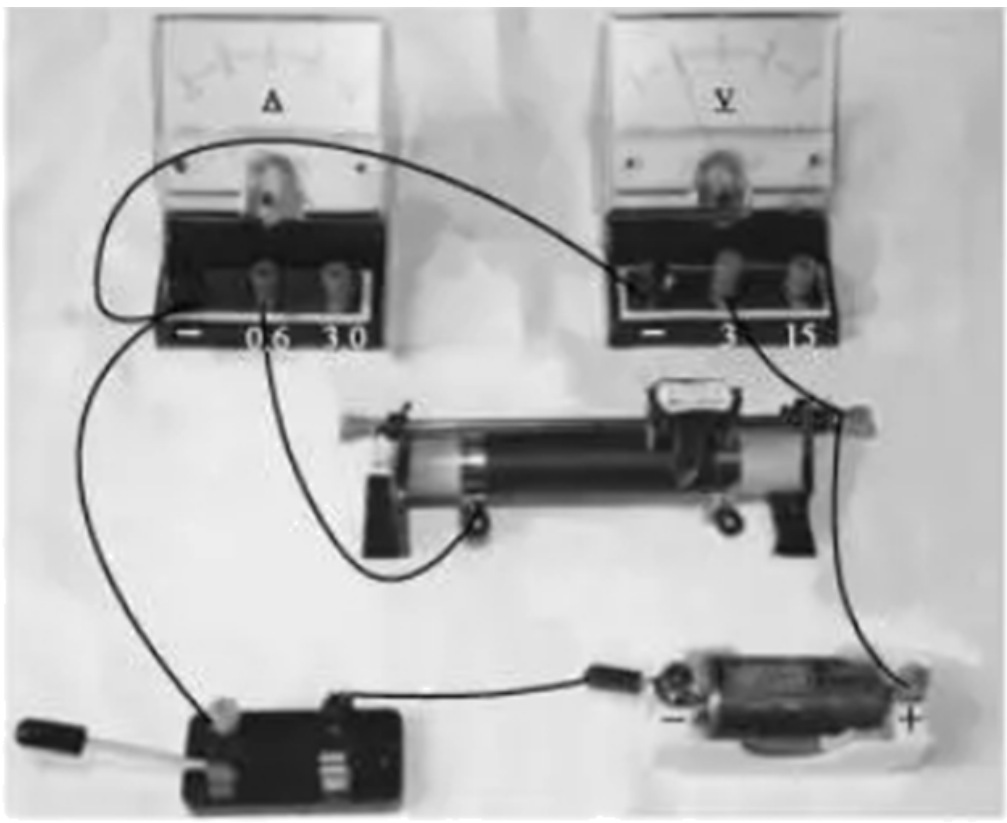
\includegraphics[width=0.9\linewidth]{picture/screenshot051}
\caption{}\label{}
\end{subfigure}
\end{figure}



\begin{enumerate}
%\renewcommand{\labelenumi}{\arabic{enumi}.}
% A(\Alph) a(\alph) I(\Roman) i(\roman) 1(\arabic)
%设定全局标号series=example	%引用全局变量resume=example
%[topsep=-0.3em,parsep=-0.3em,itemsep=-0.3em,partopsep=-0.3em]
%可使用leftmargin调整列表环境左边的空白长度 [leftmargin=0em]
\item
在答题纸相应的方框中画出图$ b $的电路图;

\item 
某次测量时电流表和电压表的示数如图所示,则电流 $ I= $ \underlinegap $A $,电压 $ U $
\underlinegap 
$ = V $;
\begin{figure}[h!]
\centering
\includesvg[width=0.33\linewidth]{picture/svg/GZ-3-tiyou-0720}
\hfil
 \includesvg[width=0.33\linewidth]{picture/svg/GZ-3-tiyou-0721} 
\end{figure}





\item 
实验得到如图所示的两条直线,图中直线$ \lmd{1} $对应电路是图 \underlinegap (选填“$ a $”或“$ b $”)
\begin{figure}[h!]
\centering
\includesvg[width=0.36\linewidth]{picture/svg/GZ-3-tiyou-0722}
\end{figure}




\item 
该电池的电动势 $ E=$ \underlinegap $V $(保留三位有效数字),内阻 $ r= $ \underlinegap $ \Omega $ (保留两位有效数字)。

\end{enumerate}


\tk{
\begin{enumerate}
%\renewcommand{\labelenumi}{\arabic{enumi}.}
% A(\Alph) a(\alph) I(\Roman) i(\roman) 1(\arabic)
%设定全局标号series=example	%引用全局变量resume=example
%[topsep=-0.3em,parsep=-0.3em,itemsep=-0.3em,partopsep=-0.3em]
%可使用leftmargin调整列表环境左边的空白长度 [leftmargin=0em]
\item
电路图:
\begin{center}
 \includesvg[width=0.6\linewidth]{picture/svg/GZ-3-tiyou-0728} 
\end{center}
\item 	
$0.39 \sim 0.41$
\item 
$1.29 \sim 1.31$
\item 
$ b $
\item 
$1.51 \sim 1.54$
\item 
$0.52 \sim 0.54$
\end{enumerate}
} 


%题目类型:
%题目区域:
%题目难度:
%思想方法:
%题目特征:

\newpage
\item
如图 $ a $所示,有一质量 $ m=200 \ kg $ 的物件在电机的牵引下从地面竖直向上经加速、匀速、匀减速至指定
位置。当加速运动到总位移的$ \frac{ 1 }{ 4 } $
时开始计时,测得电机的牵引力随时间变化的 $ F-t $ 图线如图 $ b $ 所示,$ t=34 \ s $
末速度减为 $ 0 $ 时恰好到达指定位置。若不计绳索的质量和空气阻力,求物件:
\begin{enumerate}
%\renewcommand{\labelenumi}{\arabic{enumi}.}
% A(\Alph) a(\alph) I(\Roman) i(\roman) 1(\arabic)
%设定全局标号series=example	%引用全局变量resume=example
%[topsep=-0.3em,parsep=-0.3em,itemsep=-0.3em,partopsep=-0.3em]
%可使用leftmargin调整列表环境左边的空白长度 [leftmargin=0em]
\item
做匀减速运动的加速度大小和方向;



\item 
匀速运动 的速度大小;

\item 
总位移的大小。

\end{enumerate}
\begin{figure}[h!]
\flushright 
\begin{subfigure}{0.4\linewidth}
\centering
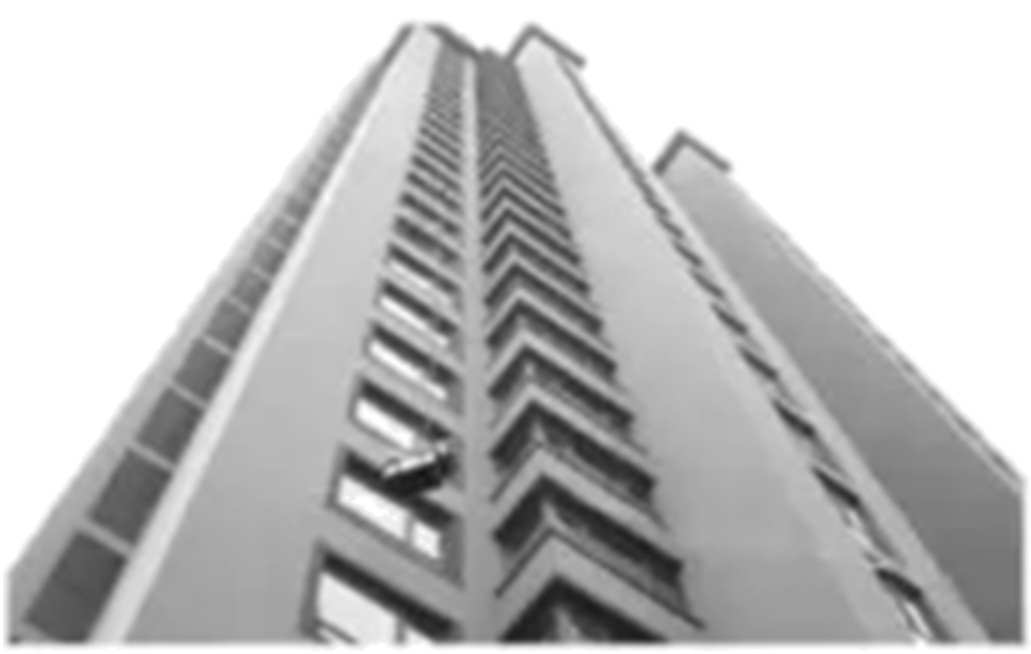
\includegraphics[width=0.7\linewidth]{picture/screenshot052}
\caption{}\label{}
\end{subfigure}
\begin{subfigure}{0.4\linewidth}
\centering
\includesvg[width=0.7\linewidth]{picture/svg/GZ-3-tiyou-0723} 
\caption{}\label{}
\end{subfigure}
\end{figure}



\banswer{
\begin{enumerate}
%\renewcommand{\labelenumi}{\arabic{enumi}.}
% A(\Alph) a(\alph) I(\Roman) i(\roman) 1(\arabic)
%设定全局标号series=example	%引用全局变量resume=example
%[topsep=-0.3em,parsep=-0.3em,itemsep=-0.3em,partopsep=-0.3em]
%可使用leftmargin调整列表环境左边的空白长度 [leftmargin=0em]
\item
$ a=0.125\ m/s^{2} $竖直向下;
\item 
$ v=1 \ m/s $;
\item 
$ x=40 \ m $	
\end{enumerate}
}



%题目类型:
%题目区域:
%题目难度:
%思想方法:
%题目特征:


\newpage
\item
小明将如图所示的装置放在水平地面上,该装置由弧形轨道、竖直圆轨道、水平直轨道 $ AB $ 和倾角
$ \theta=37 ^{ \circ } $ 的斜轨道 $ BC $ 平滑连接而成。质量 $ m=0.1 \ kg $ 的小滑块从弧形轨道离地高 $ H=1.0 \ m $ 处静止释放。已
知 $ R=0.2 \ m $, $ L_{AB}=L_{BC}=1.0 \ m $,滑块与轨道 $ AB $ 和 $ BC $ 间的动摩擦因数均为 $ \mu=0.25 $,弧形轨道和圆轨
道均可视为光滑,忽略空气阻力。
\begin{enumerate}
%\renewcommand{\labelenumi}{\arabic{enumi}.}
% A(\Alph) a(\alph) I(\Roman) i(\roman) 1(\arabic)
%设定全局标号series=example	%引用全局变量resume=example
%[topsep=-0.3em,parsep=-0.3em,itemsep=-0.3em,partopsep=-0.3em]
%可使用leftmargin调整列表环境左边的空白长度 [leftmargin=0em]
\item
求滑块运动到与圆心 $ O $ 等高的 $ D $ 点时对轨道的压力;



\item 
通过计算判断滑块能否冲出斜轨道的末端 $ C $ 点;



\item 
若滑下的滑块与静止在水平直轨道上距 $ A $ 点 $ x $ 处的质量为 $ 2m $ 的小滑块相碰,碰后一起运动,动摩擦因
数仍为 $ 0.25 $,求它们在轨道 $ BC $ 上到达的高度 $ h $ 与 $ x $ 之间的关系。(碰撞时间不计, $ \sin 37 ^{ \circ } =0.6 ,\cos 37 ^{ \circ } =0.8 $ )
\end{enumerate}
\begin{figure}[h!]
\flushright
\includesvg[width=0.45\linewidth]{picture/svg/GZ-3-tiyou-0724}
\end{figure}

\tk{
\begin{enumerate}
%\renewcommand{\labelenumi}{\arabic{enumi}.}
% A(\Alph) a(\alph) I(\Roman) i(\roman) 1(\arabic)
%设定全局标号series=example	%引用全局变量resume=example
%[topsep=-0.3em,parsep=-0.3em,itemsep=-0.3em,partopsep=-0.3em]
%可使用leftmargin调整列表环境左边的空白长度 [leftmargin=0em]
\item
$ F_{N}=8 \ N $,方向水平向左;
\item 
能在斜轨道上到达的最高点为 $C^{\prime}$ 点,由于$L_{BC^{\prime}}=\frac{15}{16} m<1$,不会冲出;
\item 
$ h=
\left\{
\begin{aligned}
	&\frac{1}{6} x-\frac{5}{48} \quad &\left(\frac{5}{8} m<x \leq 1 \ m\right)\\
	&0  \quad &\left(0 \leq x \leq \frac{5}{8} \ m\right)
\end{aligned}
\right.
 $
\end{enumerate}
} 

%题目类型:
%题目区域:
%题目难度:
%思想方法:
%题目特征:

\newpage
\item
如图 $ a $ 所示,在绝缘光滑水平桌面上,以 $ O $ 为原点、水平向右为正方向建立 $ x $ 轴,在 $ 0 \leq x \leq 1.0 \ m $ 区
域内存在方向竖直向上的匀强磁场。桌面上有一边长 $ L=0.5 \ m $、电阻 $ R=0.25 \ \Omega $ 的正方形线框 $ abcd $,当
平行于磁场边界的 $ cd $ 边进入磁场时,在沿 $ x $ 方向的外力 $ F $ 作用下以 $ v=1.0 \ m/s $ 的速度做匀速运动,直到 $ ab $
边进入磁场时撤去外力。若以 $ cd $ 边进入磁场时作为计时起点,在 $ 0 \leq t \leq 1.0 \ s $ 内磁感应强度 $ B $ 的大小与时间
$ t $ 的关系如图 $ b $ 所示,在 $ 0 \leq t \leq 1.3 \ s $ 内线框始终做匀速运动。
\begin{enumerate}
%\renewcommand{\labelenumi}{\arabic{enumi}.}
% A(\Alph) a(\alph) I(\Roman) i(\roman) 1(\arabic)
%设定全局标号series=example	%引用全局变量resume=example
%[topsep=-0.3em,parsep=-0.3em,itemsep=-0.3em,partopsep=-0.3em]
%可使用leftmargin调整列表环境左边的空白长度 [leftmargin=0em]
\item
求外力 $ F $ 的大小;



\item 
在 $ 1.0 \leq t \leq 1.3 \ s $ 内存在连续变化的磁场,求磁感应强度 $ B $ 的大小与时间 $ t $ 的关系;



\item 
求在 $ 0 \leq t \leq 1.3 \ s $ 内流过导线横截面的电荷量 $ q $。
\end{enumerate}
\begin{figure}[h!]
\flushright
\begin{subfigure}{0.44\linewidth}
\centering
\includesvg[width=0.9\linewidth]{picture/svg/GZ-3-tiyou-0725} 
\caption{}\label{}
\end{subfigure}
\hfil
\begin{subfigure}{0.5\linewidth}
\centering
\includesvg[width=0.95\linewidth]{picture/svg/GZ-3-tiyou-0726} 
\caption{}\label{}
\end{subfigure}
\end{figure}


\tk{
\begin{enumerate}
%\renewcommand{\labelenumi}{\arabic{enumi}.}
% A(\Alph) a(\alph) I(\Roman) i(\roman) 1(\arabic)
%设定全局标号series=example	%引用全局变量resume=example
%[topsep=-0.3em,parsep=-0.3em,itemsep=-0.3em,partopsep=-0.3em]
%可使用leftmargin调整列表环境左边的空白长度 [leftmargin=0em]
\item
$ F=0.0625 \ N $	
\item 
$B=\frac{1}{6-4 t}$
\item 
$ q=0.5 \ C $
\end{enumerate}
} 

%题目类型:
%题目区域:
%题目难度:
%思想方法:
%题目特征:

\newpage
\item 
某种离子诊断测量简化装置如图所示。竖直平面内存在边界为矩形 $ EFGH $、方向垂直纸面向外、磁感
应强度大小为 $ B $ 的匀强磁场,探测板 $ CD $ 平行于 $ HG $ 水平放置,能沿竖直方向缓慢移动且接地。$ a $、$ b $、$ c $三束宽度不计、间距相等的离子束中的离子均以相同速度持续从边界 $ EH $ 水平射入磁场,$ b $ 束中的离子在磁
场中沿半径为 $ R $ 的四分之一圆弧运动后从下边界 $ HG $ 竖直向下射出,并打在探测板的右边缘 $ D $ 点。已知每
束每秒射入磁场的离子数均为 $ N $,离子束间的距离均为 $ 0.6R $,探测板 $ CD $ 的宽度为 $ 0.5R $,离子质量均为
$ m $、电荷量均为 $ q $,不计重力及离子间的相互作用。
\begin{enumerate}
%\renewcommand{\labelenumi}{\arabic{enumi}.}
% A(\Alph) a(\alph) I(\Roman) i(\roman) 1(\arabic)
%设定全局标号series=example	%引用全局变量resume=example
%[topsep=-0.3em,parsep=-0.3em,itemsep=-0.3em,partopsep=-0.3em]
%可使用leftmargin调整列表环境左边的空白长度 [leftmargin=0em]
\item
求离子速度 $ v $ 的大小及 $ c $ 束中的离子射出磁场边界 $ HG $ 时与 $ H $ 点的距离 $ s $;



\item 
求探测到三束离子时探测板与边界 $ HG $ 的最大距离 $ L_{max} $;



\item 
若打到探测板上的离子被全部吸收,求离子束对探测板的平均作用力的竖直分量 $ F $ 与板到 $ HG $ 距离 $ L $ 的
关系。


\end{enumerate}
\begin{figure}[h!]
\flushright
\includesvg[width=0.25\linewidth]{picture/svg/GZ-3-tiyou-0727}
\end{figure}

\tk{
\begin{enumerate}
%\renewcommand{\labelenumi}{\arabic{enumi}.}
% A(\Alph) a(\alph) I(\Roman) i(\roman) 1(\arabic)
%设定全局标号series=example	%引用全局变量resume=example
%[topsep=-0.3em,parsep=-0.3em,itemsep=-0.3em,partopsep=-0.3em]
%可使用leftmargin调整列表环境左边的空白长度 [leftmargin=0em]
\item
$v=\frac{q B R}{m}, \quad s=0.8 R$	
\item 	
$L_{\max }=\frac{4}{15} R$
\item 
$ 
F=
\left\{
\begin{aligned}
	&2.6 NqBR   &0<L \leq \frac{4}{15} R\\
	&1.8 NqBR  &\frac{4}{15} R<L \leq 0.4 R\\
	&N q B R  &L>0.4 R
\end{aligned}
\right.
 $
\end{enumerate}
} 

%题目类型:
%题目区域:
%题目难度:
%思想方法:
%题目特征:



\end{enumerate}


